% ql.tex

\chapter{Path Selection via Reinforcement Learning}
\label{chap:ql}

Exhaustive search by Dijkstra's algorithm in chapter \ref{chap:dijkstra}, and empirical benchmarking in section \ref{sec:smcpath} have demonstrated the theoretical utility of an augmented state space. 
In practice however, the principal challenge is to efficiently navigate the augmented state space to find improved paths without offsetting the gains in efficiency afforded by those paths.
We draw on machine learning techniques from the reinforcement learning literature to address this task.

\section{SMC and the multi-armed bandit}

The multi-armed bandit problem\cite{tokic2011value, scott2010modern, vermorel2005multi} is an optimization problem originating from probability theory. 
Selecting between an enumerated set of paths for free energy estimation can be cast as a sample allocation problem, where the conflicting goals of drawing samples for estimation along the putative best path and drawing samples for estimating the quality of other potentially better paths are in opposition. 
In figure \ref{fig:aisbandit}, we examine our ability to optimize paths with SMC by comparing three bandit strategies. 

\begin{figure}
    \centering
    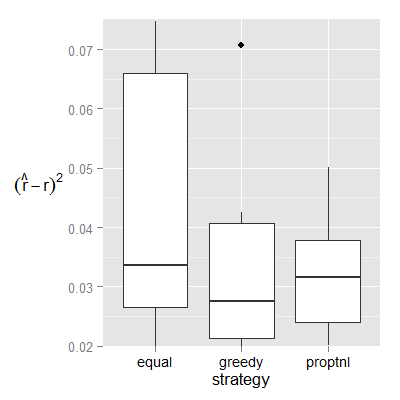
\includegraphics[scale=0.7]{ais-bandit.png}
    \caption[Comparison of three AIS bandit strategies]{Comparison of squared error for three AIS bandit strategies for offset harmonic wells. See text for details on strategies.}
    \label{fig:aisbandit}
\end{figure}

The ``equal'' strategy is effectively the null strategy, where each path is sampled equally, regardless of their estimated variances.
The ``greedy'' strategy follows up an initial exploration period of equal sampling with a period where only the minimum estimated variance path is sampled.
The ``proptnl'' strategy follows up an initial exploration period of equal sampling with a period where each path is sampled in quantities inversely proportional to their variances.
We observe that the greedy strategy is, on average, the strategy that minimizes the squared error of the ratio estimate, however it is also interesting to note that the proportional strategy is the most consistent one.

A weakness of this form of path selection, as we alluded to in section \ref{sec:pcrooks}, is that it only operates on fully predefined paths.
As we saw in figure \ref{fig:kshortest}, the shape of the optimal path can vary, and as the dimensionality of the underlying distributions increases, it is possible that the optimal paths will become more irregular in order to navigate around energetic barriers. 
In these situations, where we have no intuition to guide path definition, selection between enumerated paths may not be sufficient for the efficiency gains we seek, and a full grid optimization is required, where a path is built edge by edge.

\section{Full grid optimization with Q-learning}

Q-learning\cite{watkins1992q} is a reinforcement learning technique for finite state Markov decision processes, typically used to derive an optimal action selection policy for total reward maximization.
Q-learning progresses through successive learning episodes, where a $Q$ function describing the expected values of the long term rewards for each state-action pair is inferred via value iteration updates. Search agent actions, and the putative best path are both guided by the current best estimate of the $Q$ function, which is updated as follows after each search episode:

\begin{equation}
    Q_{t+1}(s,a) = Q_t(s,a) + \alpha (R(s,a) + \gamma \max_{a^\prime}Q_t(s^{\prime}, a^{\prime}) - Q_t(s,a))
\end{equation}

\noindent where $\alpha \in [0,1]$ is the learning rate, $\gamma \in [0,1]$ is a discount factor to penalize delayed rewards, $R(s,a)$ is a function that returns some reward for the action $a$ out of state $s$, and the maximum is the maximum $Q$ value for all actions out of the resulting state for the observed action.

In our application, as our goal is to minimize the variance of the path, the reward function $R(s,a)$, represents estimated variances for a given transition between states. 
These variance estimates are given by equation \eqref{eq:varbar} for a low cost pCrooks run.
Ratio estimates for a given transition from separate learning episodes can be combined as a mean weighted by their inverse variances.

To make Q-learning compatible with a minimization task, we make two important adjustments in order to minimize the accumulated reward.
First, we take the minimum $Q$ value over the resulting states, instead of the maximum.
Second, $\gamma$ now takes values of 1 or higher.
This second adjustment is required to avoid situations where Q-learning will create infinite loops in the solution path to delay a required large cost action. 
In a minimization context, when $\gamma$ is bounded by 0 and 1, longer paths are favored, as distal costs become discounted. 
As we've previously seen, longer paths come at a larger computational cost, so we constrain $\gamma$ to be 1 or larger, to favor shorter paths. 
$\gamma$ can be tuned to reflect the relative cost of equilibrium sampling and nonequilibrium SMC transition moves, where values near one represent low cost SMC moves.

\subsection{Fixed duration Q-learning} % (fold)
\label{sub:fixed_duration_q_learning}

In this section, Q-learning is run for a preselected number of learning episodes, representing a fixed ceiling on the amount of available computation time.
$\alpha$ is set to 0.8, and $\gamma$ is set to 1.
The search space is the augmented $(\lambda, T)$ space for the offset harmonic wells. 

\begin{figure}
    \centering
    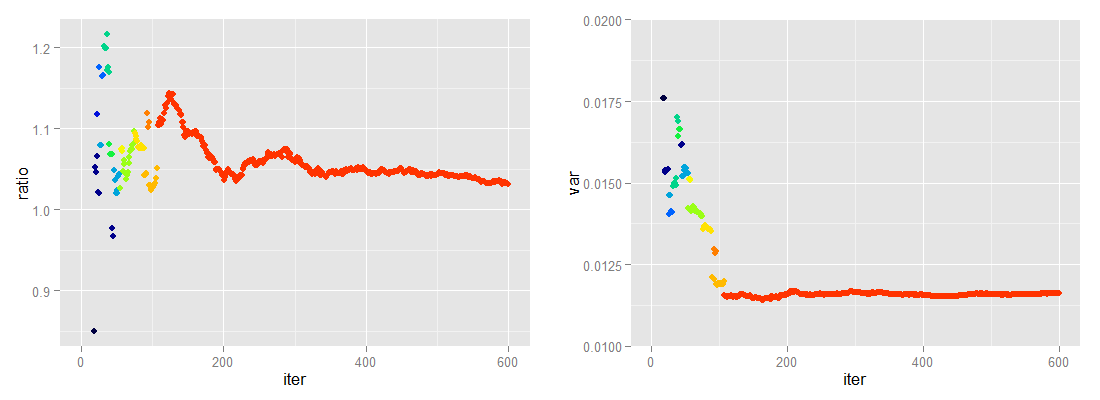
\includegraphics[scale=0.5]{ql-monitor-chain1.png}
    \caption[Ratio and variance estimates monitored for fixed duration Q-learning]{Ratio and variance estimates monitored for fixed duration Q-learning. Target distributions are offset harmonic wells, $\alpha=0.8, \gamma=1$. Changes in point color represent changes in the current best path.}
    \label{fig:ql-summary}
\end{figure}

Figure \ref{fig:ql-summary} shows the evolution of the ratio estimates, variance estimates, and current best path as a function of the number of learning episodes that have elapsed.
For the first 100 steps of the algorithm, the best guess optimal path varies rapidly, as denoted by the changing point colors.
As the algorithm progresses, path variance estimates become more precise, and the low cost paths are learned by the $Q$ function, as illustrated by the decreasing variance in the second panel, and the fixation of the red path as the optimal path.
The ratio estimation converges near the true value of 1. 

\begin{figure}
    \centering
    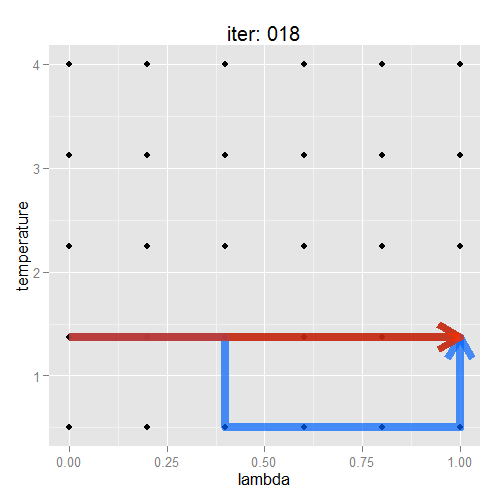
\includegraphics[scale=0.35]{iter-018.png}
    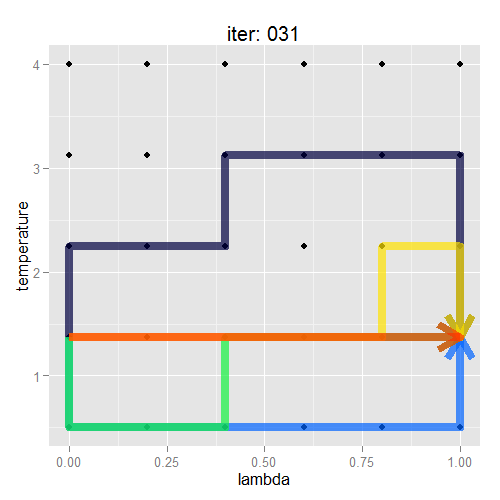
\includegraphics[scale=0.35]{iter-031.png}
    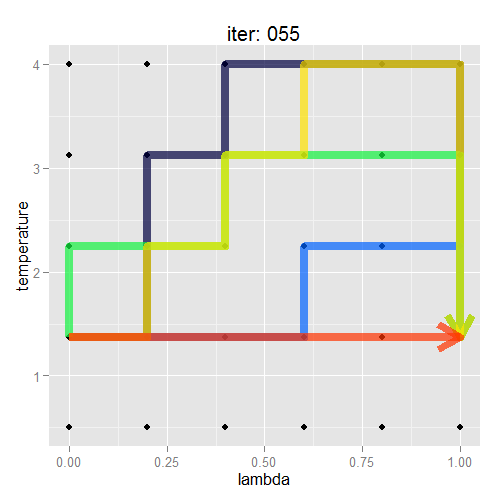
\includegraphics[scale=0.35]{iter-055.png} \\
    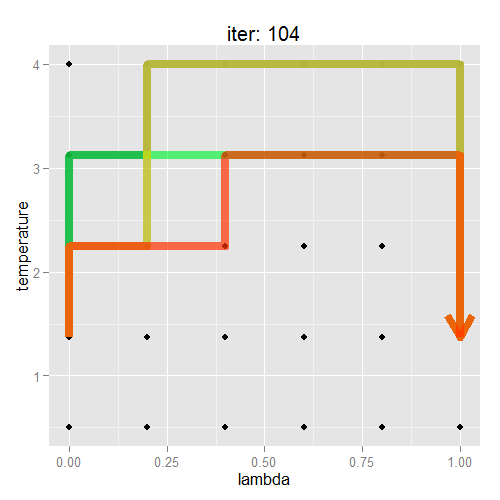
\includegraphics[scale=0.35]{iter-104.png}
    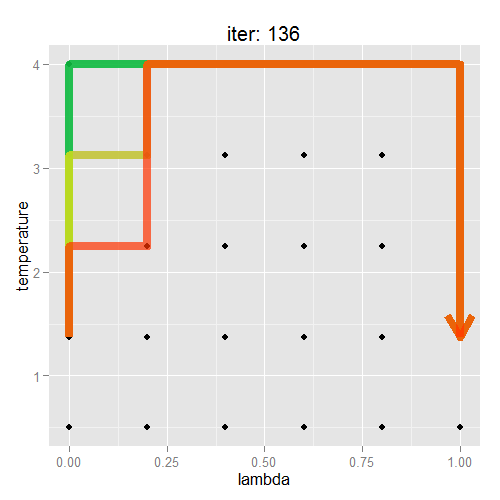
\includegraphics[scale=0.35]{iter-136.png}
    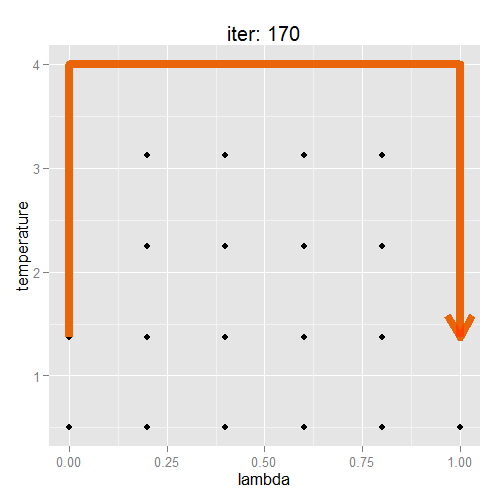
\includegraphics[scale=0.35]{iter-170.png}
    \caption[Time evolution of five Q-learning chains]{Time evolution of five Q-learning chains for offset harmonic wells. $\alpha=0.8, \gamma=1$. Each panel shows the current best path as determined by independent runs of Q-learning at different time points. Clockwise from top left: 18, 31, 55, 170, 136 and 104 iterations elapsed.}
    \label{fig:ql-slices}
\end{figure}


Figure \ref{fig:ql-slices} depicts the evolution of the best guess path for five replicates of the Q-learning algorithm on this test case.
Each color represents one chain's best guess path varying across iterations.
At the 18th iteration, only some replicates have determined a complete best path. These paths are direct, and not necessarily low variance. In fact, the path in blue is a higher variance path than the standard, fixed temperature path.
At the 31st iteration, all chains have found solution paths, but their forms vary wildly. 
Some, like the dark blue path, are promising in their use of the higher temperature regions.
By the 55th iteration, almost all paths are improved relative to the standard, fixed temperature path. 
The 104th and 136th iterations show that the chains are beginning to converge on similar solution paths. In the 136th iteration, some have even found the true optimal path we had determined by exhaustive search in figure \ref{varbar-paramviews}.
By the 170th iteration, all chains have converged on the true optimal path.
% subsection fixed_duration_q_learning (end)

\subsection{Q-learning convergence} % (fold)
\label{sub:q_learning_convergence}

The goal of a free energy calculation is to obtain an estimate of maximum precision in a set amount of time, or an estimate of set precision in a minimum amount of time.
A downside of Q-learning, and of path selection algorithms in general, is that it divides sampling efforts among many paths during the search phase, and not all of the generated SMC particles will participate in the ratio estimation if the distribution they approximate does not lie on the putative best path.
A benefit of standard $\lambda$ scaling is that all particles traverse only one path, ensuring full sample utilization, and a full reduction in variance by a factor of N.

In this section, we account for this variance reduction factor, and determine if Q-learning can converge on an improved path fast enough to offset particle waste in the early stages of the algorithm.
For both an augmented and standard state space, we run three independent Q-learning chains. 
For the standard state space, this entails simply running a free energy estimation along the fixed temperature path, as there are no alternative paths to consider.
After each iteration, we construct a composite free energy estimate based on the three chain estimates.
Within a predefined tolerance level, we assess if the individual chains agree with this composite estimate, based on a chain interval derived from the chain estimate and variance.
Chain concordance with the composite estimate provides a heuristic check for free energy estimate convergence.

\begin{figure}
    \centering
    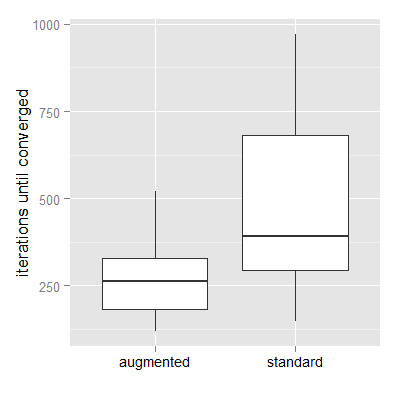
\includegraphics[scale=0.7]{ql_conv.png}
    \caption[Rates of Q-learning convergence]{Rates of Q-learning convergence for offset harmonic wells. $\alpha=0.8, \gamma=1$. For 30 replicates each, convergence rates for Q-learning in the temperature-augmented and standard state spaces are compared. The free energy estimates converge signficantly faster with path searching enabled via Q-learning, relative to when path searching is disabled, with the standard state space.}
    \label{fig:ql-convergence}
\end{figure}

The results of testing this convergence heuristic are shown in figure \ref{fig:ql-convergence}.
Despite the computational overhead Q-learning in the augmented state space incurs, it still converges significantly faster and at a more consistent rate than free energy estimation along the standard path.
On average, when path searching is permitted, convergence is achieved 1.8 times faster than when free energy estimation is confined to a fixed temperature path.
This result shows that path selection by Q-learning, in conjunction with free energy estimation with pCrooks is a valid approach for practical path optimization.

% subsection q_learning_convergence (end)
